\documentclass[
%% TIKZ_CLASSOPTION %%
tikz
]{standalone}
\usepackage{amsmath}
\usetikzlibrary{matrix}
%% EXTRA_TIKZ_PREAMBLE_CODE %%
\begin{document}
%% TIKZ_CODE %%
\begin{figure}[htbp]
    % Subfigure 1
    \begin{subfigure}[t]{0.48\textwidth}
        \centering
        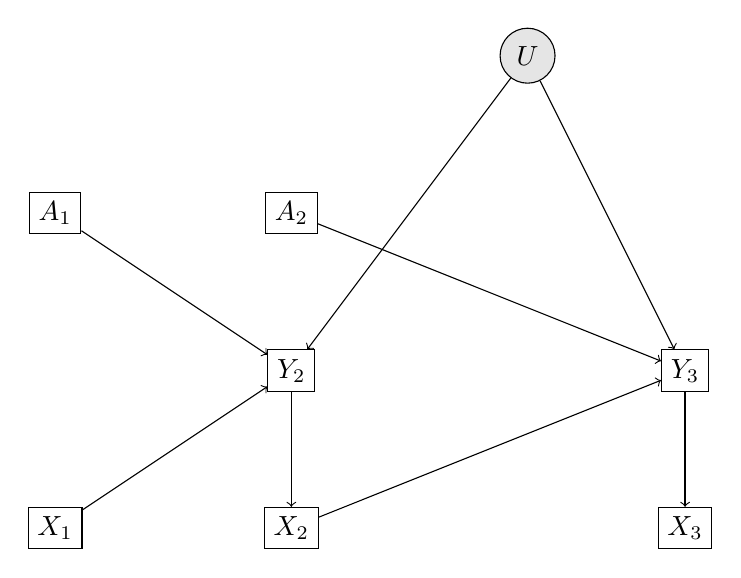
\begin{tikzpicture}
          % Nodes for observed variables (squares)
          \node[draw, rectangle] (X1) at (0, -2) {$X_{1}$};
          \node[draw, rectangle] (A1) at (0, 2) {$A_{1}$};
          \node[draw, rectangle] (Y2) at (3, 0) {$Y_{2}$};
          \node[draw, rectangle] (X2) at (3, -2) {$X_{2}$};
          \node[draw, rectangle] (A2) at (3, 2) {$A_{2}$};
          \node[draw, rectangle] (Y3) at (8, 0) {$Y_{3}$};
          \node[draw, rectangle] (X3) at (8, -2) {$X_{3}$};

          % Node for latent variable (circle)
          \node[draw, circle, fill=gray!20] (U) at (6, 4) {$U$};

          % Directed edges
          \draw [->] (U) -- (Y2);
          \draw [->] (U) -- (Y3);
          \draw [->] (A2) -- (Y3);
          \draw [->] (X2) -- (Y3);
          \draw [->] (Y2) -- (X2);
          \draw [->] (A1) -- (Y2);
          \draw [->] (X1) -- (Y2);
          \draw [->] (Y3) -- (X3);
        \end{tikzpicture}
        \caption{Generative Model 1}
        \label{fig:GM1_DAG}
    \end{subfigure}
    \hfill
    % Subfigure 2
    \begin{subfigure}[t]{0.48\textwidth}
        \centering
        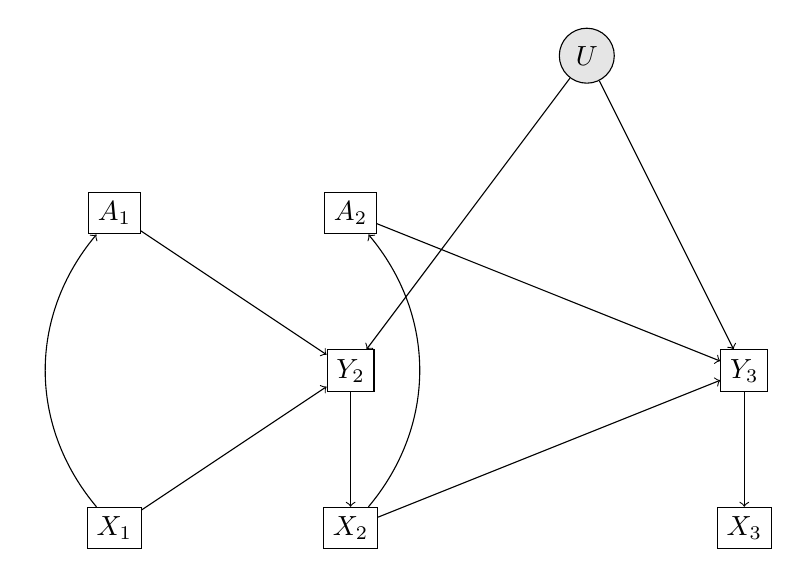
\begin{tikzpicture}
          % Nodes for observed variables (squares)
          \node[draw, rectangle] (X1) at (0, -2) {$X_{1}$};
          \node[draw, rectangle] (A1) at (0, 2) {$A_{1}$};
          \node[draw, rectangle] (Y2) at (3, 0) {$Y_{2}$};
          \node[draw, rectangle] (X2) at (3, -2) {$X_{2}$};
          \node[draw, rectangle] (A2) at (3, 2) {$A_{2}$};
          \node[draw, rectangle] (Y3) at (8, 0) {$Y_{3}$};
          \node[draw, rectangle] (X3) at (8, -2) {$X_{3}$};

          % Node for latent variable (circle)
          \node[draw, circle, fill=gray!20] (U) at (6, 4) {$U$};

          % Directed edges
          \draw [->] (U) -- (Y2);
          \draw [->] (U) -- (Y3);
          \draw [->] (A2) -- (Y3);
          \draw [->] (X2) -- (Y3);
          \draw [->] (Y2) -- (X2);
          \draw [->] (A1) -- (Y2);
          \draw [->] (X1) -- (Y2);
          \draw [->] (Y3) -- (X3);

          % Curved edges for X1 -> A1 and X2 -> A2
          \draw [->, bend left=40] (X1) to (A1);
          \draw [->, bend right=40] (X2) to (A2);
        \end{tikzpicture}
        \caption{Generative Model 2}
        \label{fig:GM2_DAG}
    \end{subfigure}
    \vspace{1em}
    % Subfigure 3
    \begin{subfigure}[t]{0.48\textwidth}
        \centering
        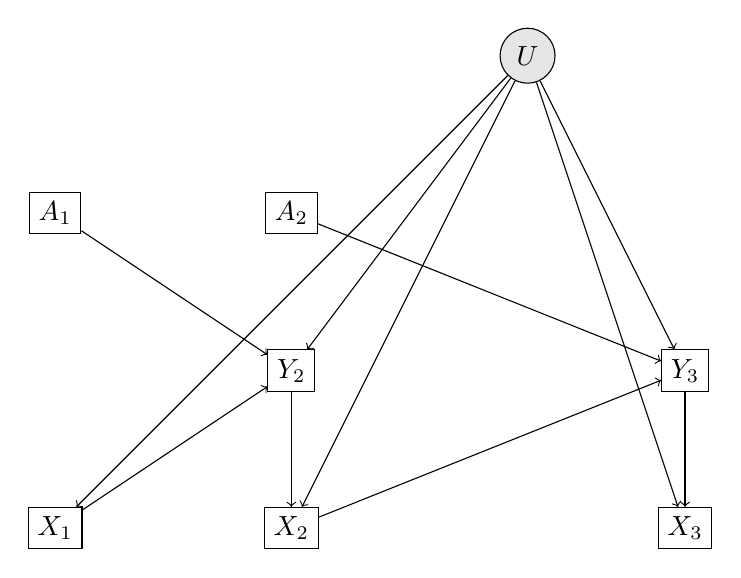
\begin{tikzpicture}
          % Nodes for observed variables
          \node[draw, rectangle] (X1) at (0, -2) {$X_1$};
          \node[draw, rectangle] (A1) at (0, 2) {$A_1$};
          \node[draw, rectangle] (Y2) at (3, 0) {$Y_2$};
          \node[draw, rectangle] (X2) at (3, -2) {$X_2$};
          \node[draw, rectangle] (A2) at (3, 2) {$A_2$};
          \node[draw, rectangle] (Y3) at (8, 0) {$Y_3$};
          \node[draw, rectangle] (X3) at (8, -2) {$X_3$};

          % Latent variable
          \node[draw, circle, fill=gray!20] (U) at (6, 4) {$U$};

          % Edges
          \draw [->] (U) -- (Y2);
          \draw [->] (U) -- (Y3);
          \draw [->] (U) -- (X1);
          \draw [->] (U) -- (X2);
          \draw [->] (U) -- (X3);
          \draw [->] (A1) -- (Y2);
          \draw [->] (X1) -- (Y2);
          \draw [->] (Y2) -- (X2);
          \draw [->] (A2) -- (Y3);
          \draw [->] (X2) -- (Y3);
          \draw [->] (Y3) -- (X3);
        \end{tikzpicture}
        \caption{Generative Model 3}
        \label{fig:GM3_DAG}
    \end{subfigure}
    \caption{DAGs for Generative Models 1, 2, and 3. Each subfigure corresponds to a distinct model configuration.}
    \label{fig:combined_DAGs}
\end{figure}
\end{document}
